\chapter{Evoluindo uma plataforma de rede social}
\label{evol-rede-social}

Neste capítulo é apresentado a plataforma Noosfero desde sua arquitetura até os processos de desenvolvimento da comunidade. Além disso é exibido o Comunidade.UnB, rede de colaboração livre, no qual são propostas evoluções para que se torne um ambiente híbrido utilizado por professores e alunos.

\section{Noosfero}
\label{noosfero}

O Noosfero \footnote{Disponível em: \url{http://www.noosfero.org}} é uma plataforma livre para criação de redes sociais desenvolvida em 2007 pela Cooperativa de Tecnologias Livres - Colivre \footnote{\url{http://www.colivre.coop.br}}, sob a licença AGPL\footnote{Licença de software GNU Affero General Public License} V3, com a proposta de facilitar a criação de redes sociais personalizadas, livres e autônomas e a geração de conteúdo colaborativo.

A Colivre é uma cooperativa sediada em Salvador/BA e contribui com a difusão e o desenvolvimento de tecnologias livres. Atualmente os desenvolvedores da Colivre realizam a manutenção e evolução do Noosfero além de manter seu repositório. Ou seja, são responsáveis por revisar os códigos que são enviados pela comunidade e integrar ao código da plataforma.

Além das funcionalidades de rede social, com foco na produção e compartilhamento de conteúdo, o Noosfero permite que dentro da rede cada usuário e comunidade tenha o seu espaço com total flexibilidade de personalização visual e gerenciamento de conteúdo. São exemplos de portais que utilizam o Noosfero: o Participa BR \footnote{\url{https://www.participa.br/}}, Stoa\footnote{\url{http://stoa.usp.br/}}, Portal da FGA\footnote{\url{http://fga.unb.br/}} e o novo Portal do Software público Brasileiro \footnote{\url{Disponível em: https://beta.softwarepublico.gov.br/}}(até então em fase \textit{beta}).

O Noosfero foi desenvolvido na linguagem de programação Ruby, atualmente na versão 2.2.0, e utiliza o \textit{framework} aplicações web \textit{Ruby on Rails} \footnote{\url{http://rubyonrails.org/}}, versão 3.2.21. E utiliza também padrões arquiteturais de software Model-View-Controller (MVC), e o padrão de plugins que serão apresentados na seção \ref{arquitetura}.

A escolha da linguagem \textit{Ruby} foi decisiva no Noosfero, pois possui uma sintaxe simples, que facilita a manutenibilidade do sistema, característica importante em projetos de software livre que tendem a atrair colaboradores externos, de acordo com \citeonline{meirelles2013}. A escolha do \textit{Rails} foi influenciada pelos seus conceitos básicos que auxiliam em sua produtividade: "Não Repita a Si Mesmo" (DRY-\textit{Don't Repeat Yourself}) e "convenção sobre configuração" (\textit{convention over configuration}) \cite{akita2006repensando}.

Por questões de segurança o Noosfero utiliza apenas pacotes \textit{stable} do \textit{Debian}, incluindo do \textit{Ruby on Rails}, por serem reconhecidos por sua estabilidade e testados sob a ótica de segurança, antes de seu lançamento. Dessa forma uma vez que a vulnerabilidade é corrigida no Debian, não é preciso corrigir no Noosfero.

\subsection{Processos e desenvolvimento da comunidade}
\label{proc-desenvol-comunidade}
% - ciclos
% - repositorio
% - commiters/revisao
% - testes

Para que novos desenvolvedores colaborem com o Noosfero a comunidade utiliza em seu próprio \textit{site} uma seção para o desenvolvimento. Nesta seção tem-se manuais com os passos para instalação do ambiente, descrição dos \textit{plugins} disponíveis, instruções para a personalização da plataforma através de temas além de informações arquiteturais da platafroma. Para realizar o controle de itens a fazer, como a implementação de novas funcionalidades ou correção de bugs é utilizado um \textit{Issue Tracker} do repositório oficial que encontra-se no GitLab.

Uma vez que o desenvolvedor tenha registro no GitLab da comunidade é possível utilizar o \textit{Issue Tracker} para cadastrar novas funcionalidades ou \textit{bugs} de maneira simples seguindo os seguintes passos:

\begin{enumerate}
\item preencher o campo título;
\item definir a descrição do item, se existir, é necessário especificar com qual \textit{plugin} o item está relacionado;
\item associar um desenvolvedor responsável pela sua implementação \textit{issue};
\item definir as \textit{labels} da funcionalidade, onde é especificado ao que está relacionado a nova \textit{issue}.
\end{enumerate}

Após a criação da \textit{issue} todos os membros da comunidade podem visualizar os dados e especificações e discutir sobre os propósitos e formas de implementação da funcionalidade.

A figura \ref{issue-tracker} evidencia o \textit{Issue Tracker} do Noosfero onde é possível verificar os itens que foram mapeados e seus respectivos \textit{status}, se ainda estão abertas ou fechadas, além de um filtro para os autores e os marcadores envolvidos à cada uma delas. Dessa forma, é possível priorizar os itens identificados como sendo de maior importância para os usuários e desenvolvedores.

\begin{figure}[h]
    \centering
    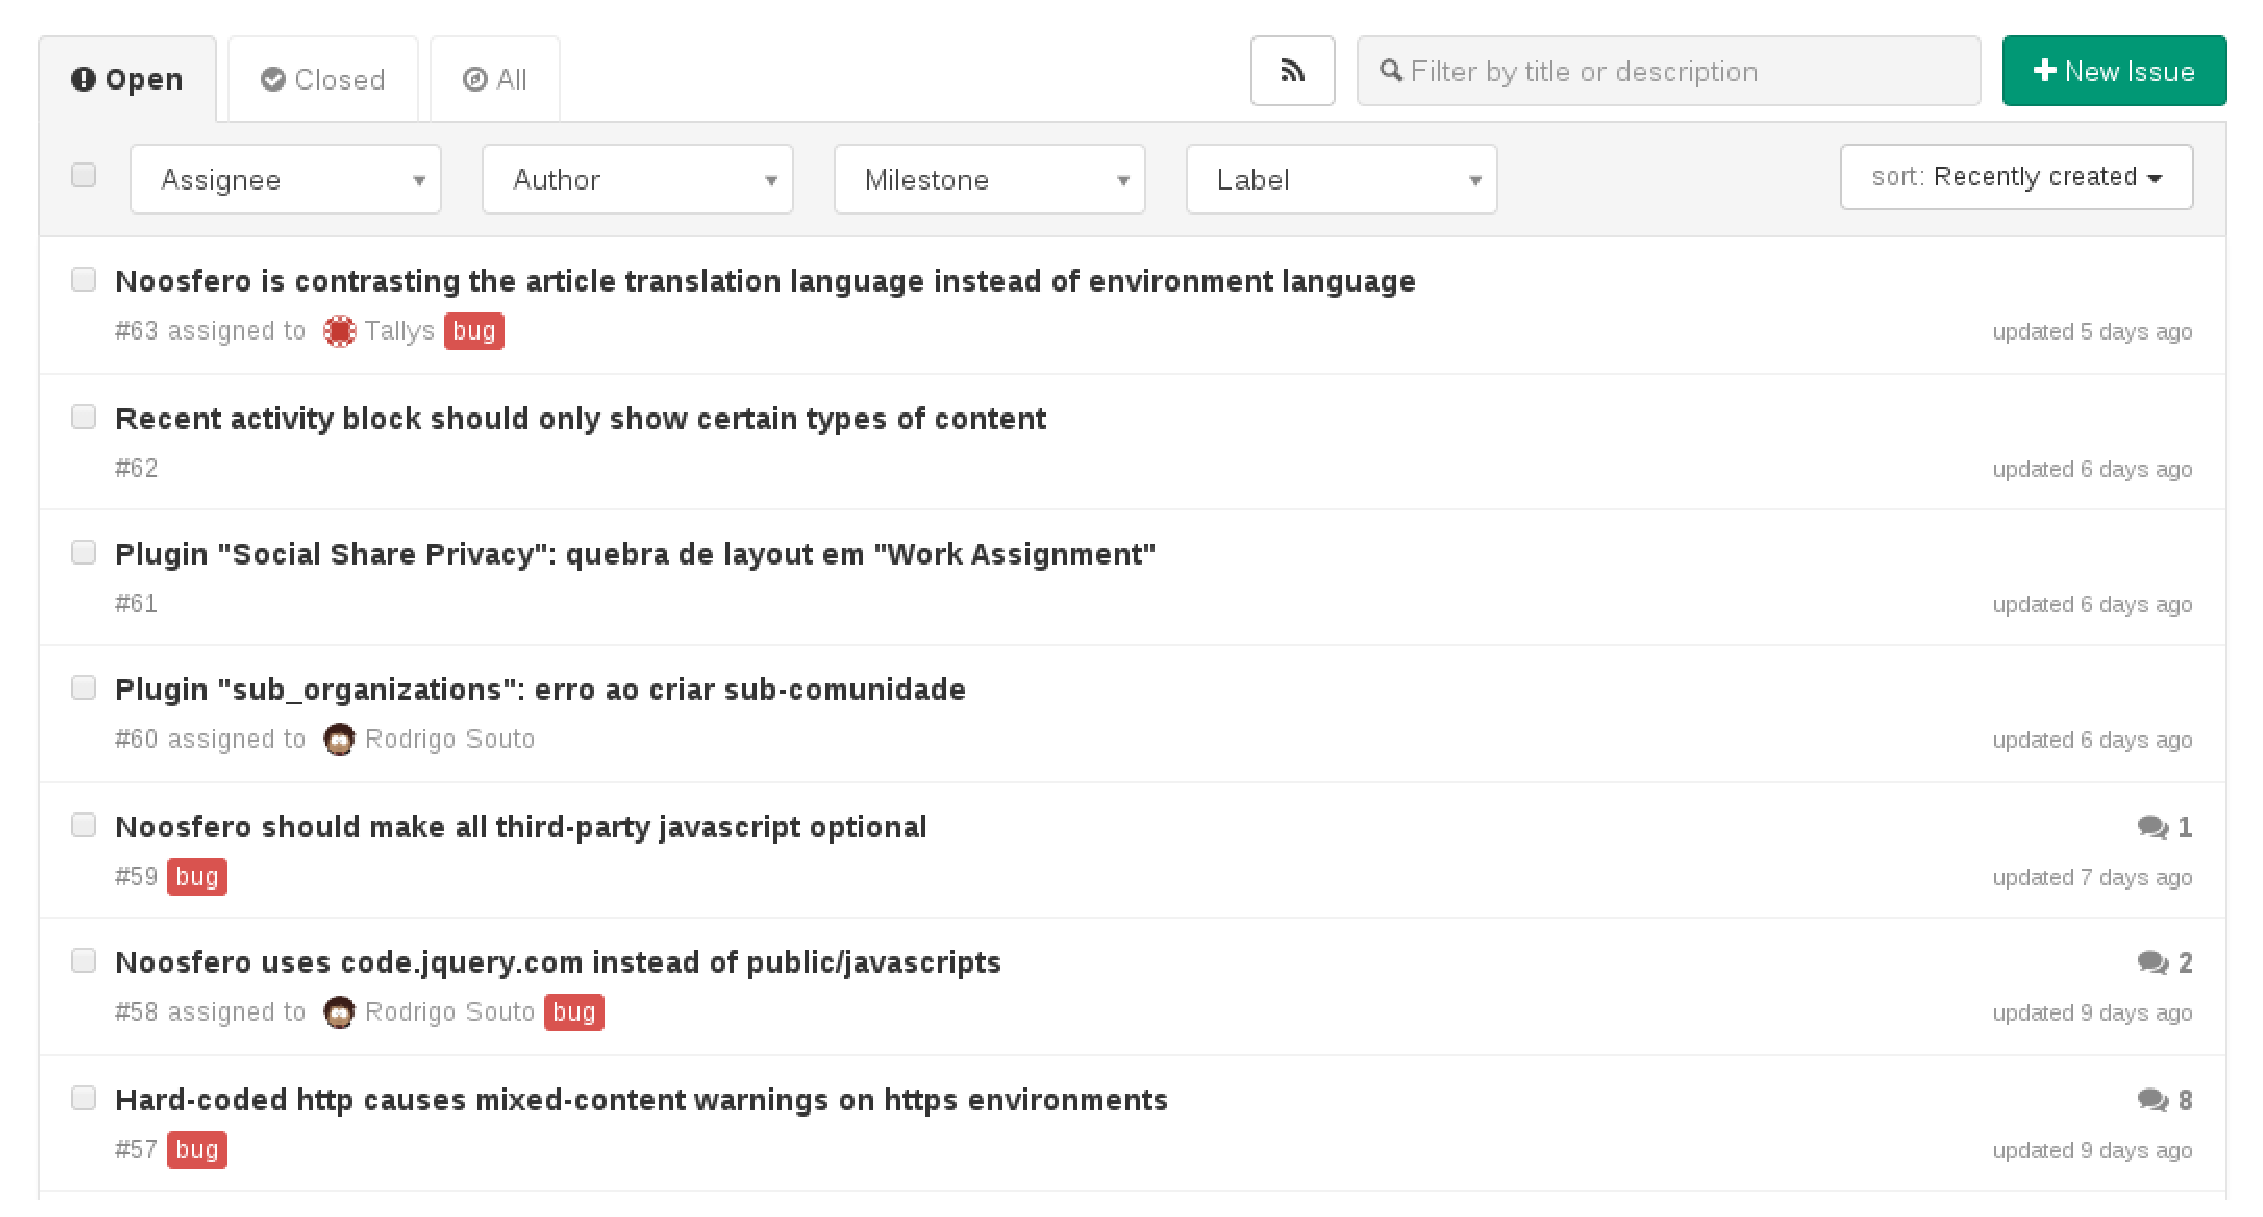
\includegraphics[keepaspectratio=true,scale=0.4]
      {figuras/issueTrackerGitLab.eps}
    \caption{Issue Tracker no GitLab}
    \label{issue-tracker}
\end{figure}

Priorizando a comunicação entre os desenvolvedores, a comunidade compartilha canais de comunicação pelo IRC (\textit{Internet Relay Chat}). Nestes os desenvolvedores podem compartilhar conhecimento e realizarem discussões técnicas sobre as implementações.

A implementação é realizada pelo desenvolvedor que tem a responsabilidade de manter a qualidade do código produzido bem como realizar todos os testes relacionados à funcionalidade implementada. Uma vez que este primeiro passo esteja concluído o código é submetido a um \textit{merge-request} onde um dos desenvolvedores do \textit{core} efetua a revisão para verificar se está de acordo com os padrões esperados, e aprova ou não, a inclusão do código na \textit{branch} principal do Noosfero.

% Retirar esse parágrafo
A comunidade Noosfero recomenda práticas de desenvolvimento como o TDD, \textit{Test Driven Development} ou Desenvolvimento orientado a testes), combinado com o BDD \footnote{\url{https://cukes.info/}} (\textit{Behavior Driven Development} ou Desenvolvimento Guiado por Comportamento, que auxiliar o desenvolvedor a criar testes e integrar regras de negócio com a linguagem de programação, mantendo o foco no comportamento do software \cite{north2006introducing}.

Para realizar o controle de versão e gerenciamento do código fonte é utilizado o \textit{Git}, uma ferramenta livre de versionamento distribuído de código fonte. O repositório oficial do Noosfero encontra-se no software livre Gitlab\footnote{\url{https://gitlab.com/noosfero/noosfero}} com um espelho no Github\footnote{\url{https://github.com/noosfero/noosfero}}. Na página de desenvolvimento da comunidade existe uma série de recomendações sobre o envio de \textit{patches} para o Noosfero, incluindo como versionamentos e solicitações de inclusão de seu \textit{patch}, ou \textit{merge-request}.

\subsection{Arquitetura}
\label{arquitetura}
 % Falar porque é importante conhecer a arquitetura do noosfero
Para a evolução de um software de forma adequada é importante o conhecimento da arquitetura do sistema, para não comprometer todo o planejamento realizado na concepção do projeto. Desse modo conhecer e entender a arquitetura de funcionamento do Noosfero é uma etapa fundamental para o densevolvimento de novas funcionalidades para a plataforma.

 % Conceitos sobre o que é arquitetura
Arquitetura de software são as estruturas do sistema, que abrange os componentes de software, as propriedades externamente visíveis desses componentes e as relações entre elas \cite{pressman2011engenharia}. De acordo com \citeonline{garlan1995introduction} a arquitetura é a estrutura dos componentes de um programa/sistema, suas inter-relações e princípios e diretrizes que regem sua concepção expondo as dimensões através das quais um sistema deve evoluir.

Apesar da existência de variações quanto à definição de arquitetura de software, entende-se que ela está ligada aos módulos do sistema e como eles se relacionam, dessa maneira todos os sistemas possuem algum tipo de arquitetura.

Na Figura \ref{arquitetura-noosfero}, é apresentado uma visão alto nível da arquitetura do Noofero. Basicamente tem-se uma arquitetura cliente-servidor onde o cliente via \textbf{\textit{Browser}} solicita um conteúdo ou uma função para o servidor Noosfero, que aguarda requisições de entrada para processá-las e compartilhar recursos com o cliente.

\begin{figure}[h]
    \centering
    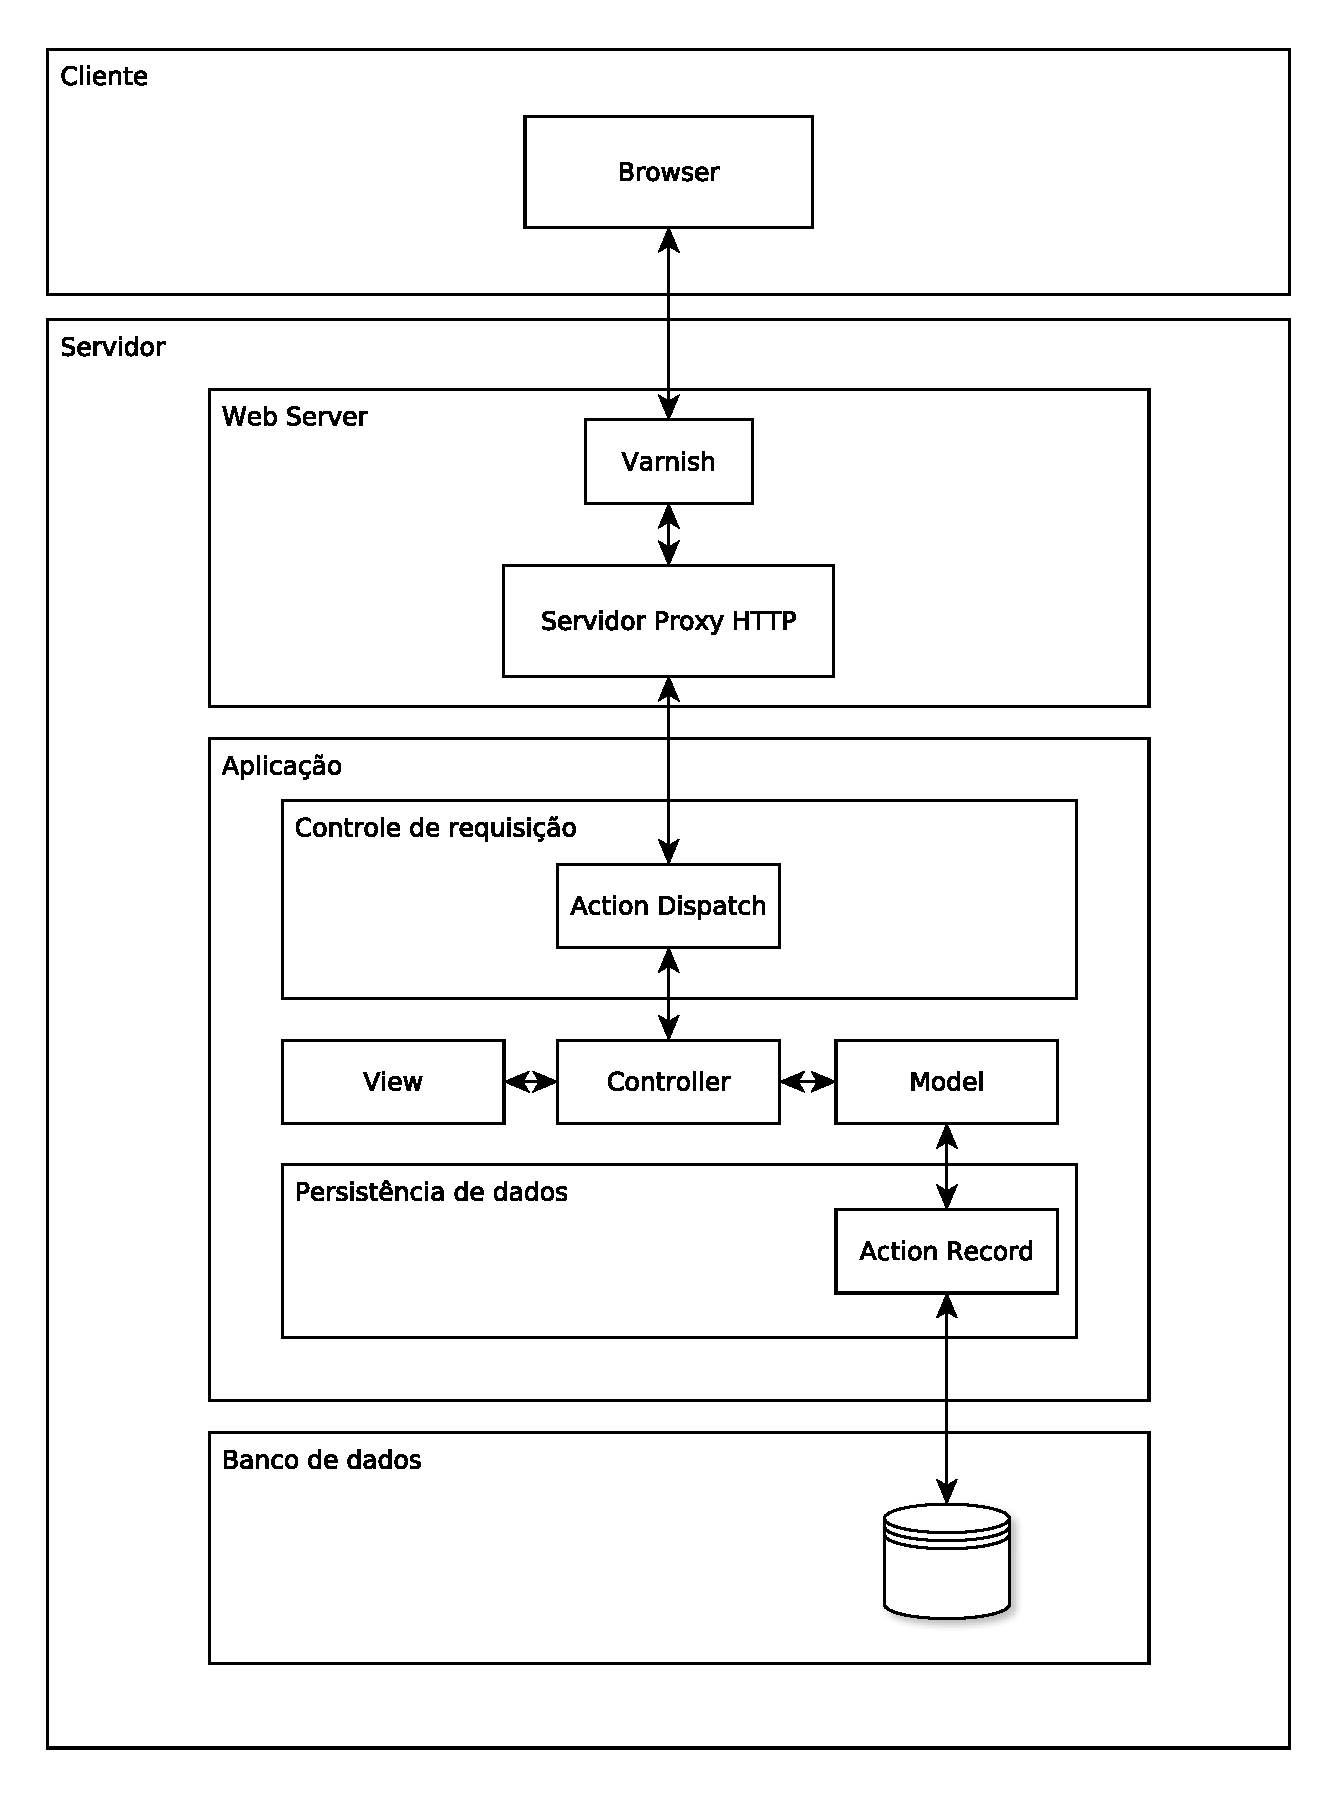
\includegraphics[keepaspectratio=true,scale=0.4]
      {figuras/DiagramaDeArquitetura.eps}
    \caption{Arquitetura do Noosfero}
    \label{arquitetura-noosfero}
\end{figure}

Do lado do servidor temos basicamente três camadas de abstração: \textit{Web-Server}, \textit{aplicação} e \textit{Banco de dados}. Na primeira camada temos dois componentes responsáveis por processar e acelerar todas as requisições de entrada e saída:

\begin{itemize}
\item Varnish: é um acelerador para sites web dinâmicos com alto volume de conteúdo que utiliza \textit{proxy} HTTP Reverso. Sua efiência deve-se ao fato dele armazenar o conteúdo HTTP requisitado na memória RAM, fazendo com que o servidor não consulte e processe diversas vezes o mesmo conteúdo solicitado.
\item Servidor Proxy HTTP: pode ser utilizado o Apache ou Nginx \footnote{\url{http://nginx.org}} que ajudam a melhorar o desempenho funcionando como um servidor proxy HTTP reverso que processa as requisições de entrada e saída e as encaminha para a aplicação executá-las.
\end{itemize}

Na camada da aplicação foi considerada uma camada responsável pelo controle de requisições, que é efetuada pelo componente \textbf{\textit{Action Dispatch}}, que lida com o mapeamento de todas as requisições, \textit{cookies} e sessão para suas respectivas \textit{controllers}.

Na aplicação utiliza-se o padrão de arquitetura de software MVC\footnote{Model-view-controller} onde a \textbf{\textit{controller}} controla o fluxo da aplicação,relacionando as entidades de \textit{model} e de \textit{view} através de chamadas de métodos. A \textbf{\textit{model}} representa as entidades do domínio da aplicação, onde a lógica do sistema são implementadas. A \textbf{\textit{view}} é a interface de comunicação com o usuário, ou seja as páginas HTML apresentadas no navegador.

Ainda na camada da aplicação tem-se o \textbf{\textit{Active Record}} que é um ORM \footnote{object-relational mapping}, um mapeador entre objetos e registros de uma tabela, onde cada classe de modelo possui uma tabela correspondente à ela no banco de dados.

Por fim temos a camada de banco de dados que recebe requisições da camada de persistência de dados e por meio de um sistema gerenciador de banco de dados (SGBD) realizam operações na base de dados.

\subsection{Modelo de domínio}

Para \citeonline[p. 160]{larman2002utilizando}, um modelo de domínio é a representação visual de classes conceituais ou objetos do mundo real em um domínio, que também podem ser chamados de modelos conceituais, modelos de objetos de domínio e modelos de objetos de análise. Dessa forma, é necessário o seu entendimento para realizar a evolução da plataforma.

O Noosfero é uma plataforma que tem suporte a vários ambientes de rede social dentro de uma mesma instalação. A Figura \ref{domain_main} mostra-se o funcionamento geral do Noosfero com suas quatro principais classes \textbf{\textit{Domain}}, \textbf{\textit{Environment}}, \textbf{\textit{Profile}} e \textbf{\textit{Article}} (Em português: Domínio, Ambiente, Perfil e Artigo respectivamente). Analisando o modelo verifica-se que na implementação é necessário que exista pelo um domínio e partir disso é possível criar várias instâncias de Ambiente na aplicação.

\begin{figure}[h]
    \centering
    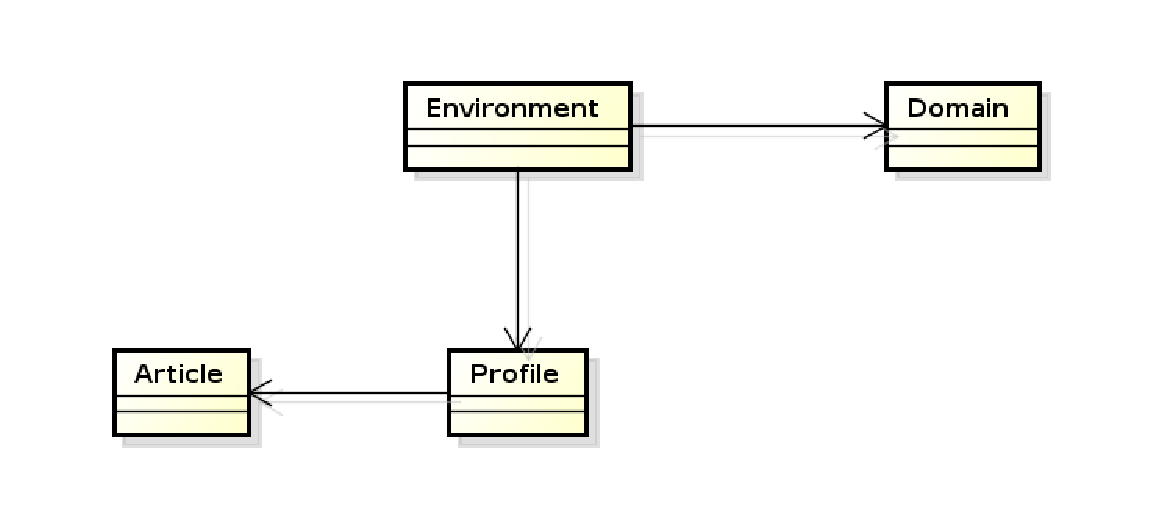
\includegraphics[keepaspectratio=true,scale=0.65]
      {figuras/domain_main.eps}
    \caption{Relações entre entidades de domínio ambiente, domínio e perfis. Extraído de: \cite{bucher2013rede}}
    \label{domain_main}
\end{figure}

A entidade Profile é uma generalização das entidades \textbf{\textit{Person}} (Pessoa) e \textbf{\textit{Organization}} (Organização), como pode ser visto na Figura \ref{domain_profiles}. Nesse mesmo modelo percebe-se que Organization é especializada nas entidades concretas \textbf{\textit{Community}} (Comunidade e Enterprise (Empreendimento). A herança é um mecanismo pelo qual qual uma classe sub-classe pode estender uma super-classe, onde basicamente isola-se métodos ou atributos em comum dentro de uma classe pai (super-classe), enquanto as especialidades são responsabilidade das classes filhas (sub-classe).

%Procurar fonte para herança
Por questões de design do código da aplicação foi criada uma entidade \textbf{\textit{User}}, ou Usuário, que é mantida separada da entidade Pessoa, que é quem implementa a lógica de autenticação da aplicação. Desta forma a lógica de autenticação fica separada da lógica de visualização e personalização do perfil.

\begin{figure}[h]
    \centering
    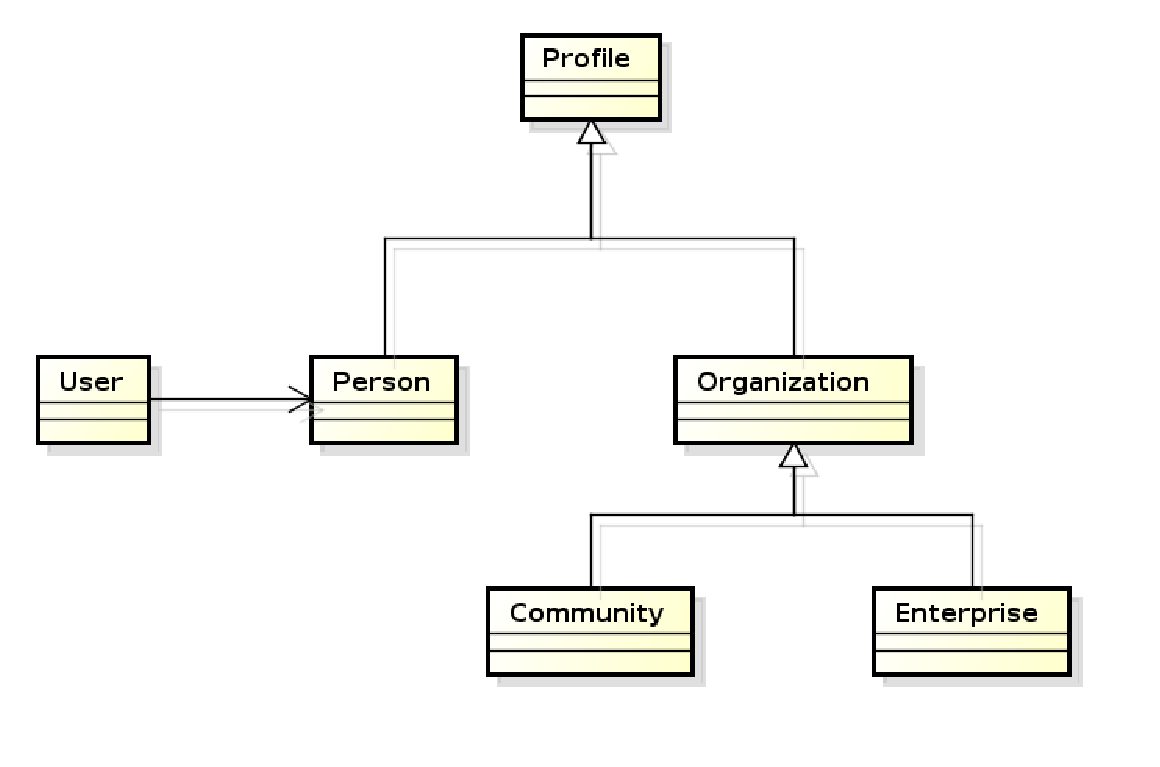
\includegraphics[keepaspectratio=true,scale=0.6]
      {figuras/domain_profiles.eps}
    \caption{Entidades de domínio: tipos de perfis. Extraído de: \cite{bucher2013rede}}
    \label{domain_profiles}
\end{figure}

Por fim, as entidades mostradas na Figura \ref{domain_articles} representam os principais tipos de conteúdos disponíveis no Noosfero, onde a classe \textbf{\textit{Article}}, ou Artigo, é uma especialização de todos os conteúdos disponíveis como: artigos de texto, pastas, blogs, galerias de imagens, fórum, arquivos e feeds de notícias.

\begin{figure}[h]
    \centering
    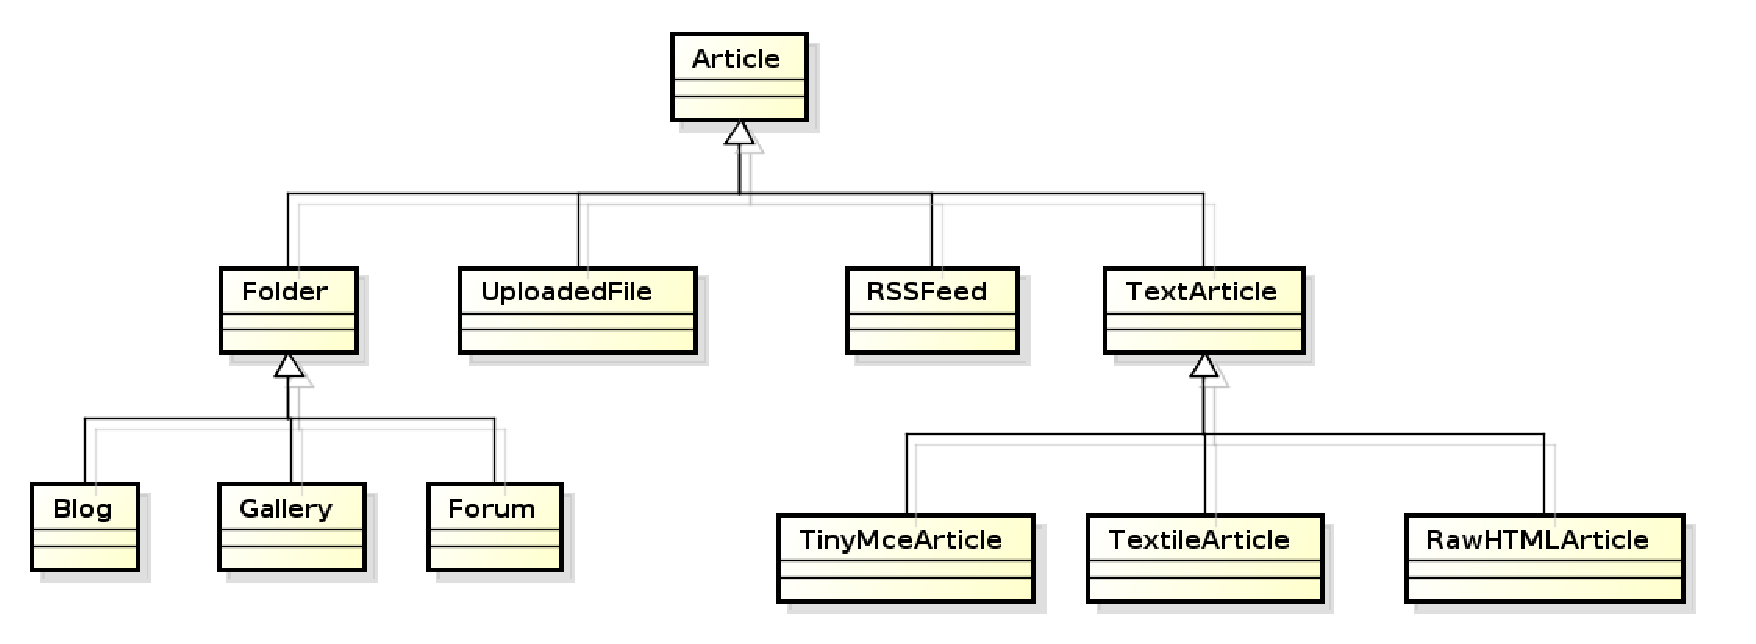
\includegraphics[keepaspectratio=true,scale=0.55]
      {figuras/domain_articles.eps}
    \caption{Entidades de domínio: tipos de artigos. Extraído de: \cite{bucher2013rede}}
    \label{domain_articles}
\end{figure}

O modelo de domínio aqui apresentado contempla o \textit{core} do noosfero. Para o acréscimo de melhorias e funcionalidades é necessário compreender a visão arquitetural dos \textit{plugins} d a plataforma, que será abordado na próxima seção.

\subsection{Plugins}

Como um software está em constante evolução a arquitetura do Noosfero foi criada para ser altamente expansível, fazendo-se o uso de \textit{plugins}. Essa arquitetura permite que em cada ambiente fique a critério do usuário quais os \textit{plugins} ou novas funcionalidades serão habilitadas, o que torna o sistema flexível e modular.

\begin{figure}[h]
    \centering
    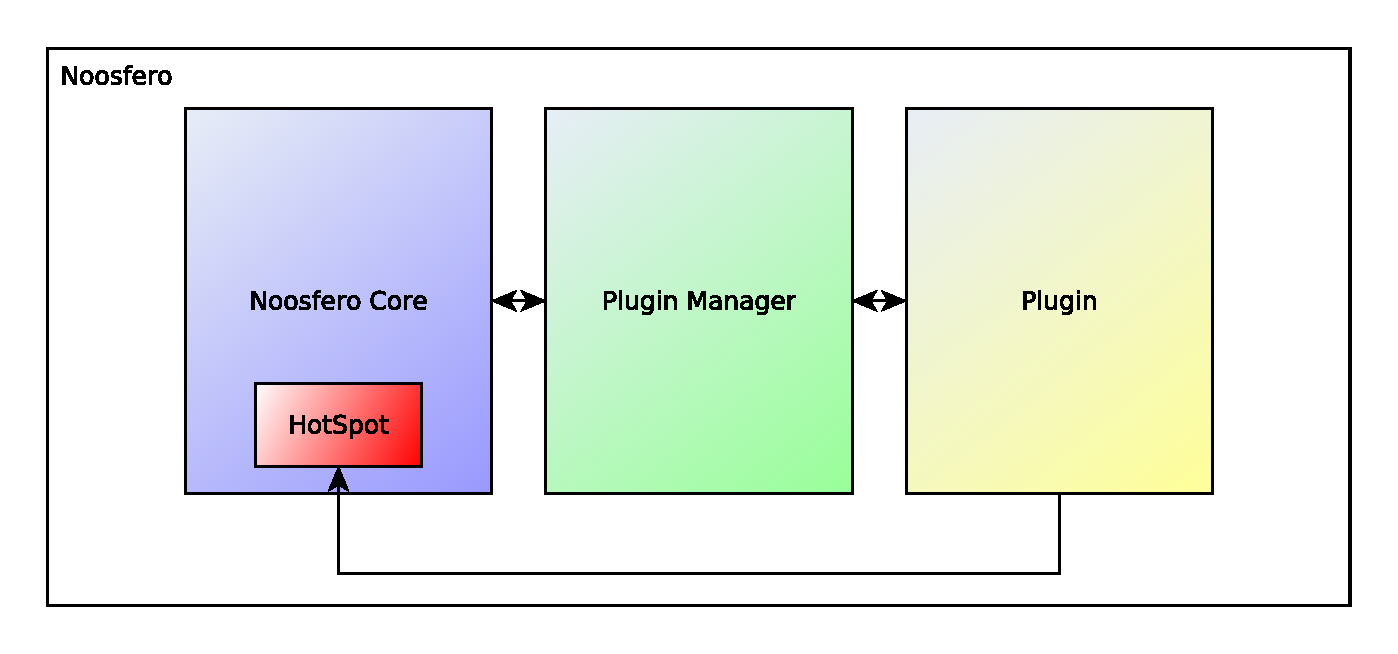
\includegraphics[keepaspectratio=true,scale=0.4]
      {figuras/estruturaDePlugins.eps}
    \caption{Estrutura de Plugins}
    \label{estrutura-plugins}
\end{figure}

A figura \ref{estrutura-plugins} é uma abstração alto nível do funcionamento interno dos plugins no Noosfero. No \textit{core} do Noosfero temos os \textit{hotspots}, que são pontos de flexibilidade que permitem associar diferentes comportamentos na execução do sistema, permitindo a inserção de trechos de código e ou alteração de um determinado método sem comprometer suas funcionalidades básicas.

Os \textit{hotspots} são gerenciados por uma camada de abstração denominada \textit{Plugin Manager}, ou Gerenciador de \textit{Plugins}, que são chamadas pelo \textit{core} através de um metódo principal conhecido como \textit{dispatch}. Basicamente o ciclo de execução pode ser descrito da seguinte maneira: durante a execução de alguma funcionalidade o método \textit{dispatch} é invocado por alguma funcionalildade do core, deste modo o gerenciador de plugins verifica todos os \textit{Plugins} que fazem uso daquele \textit{hotspot} e encaminha para cada um deles a execução de suas ações de acordo com sua implementação.

Essa arquitetura extensível adotada pelo Noosfero auxilia no controle da qualidade de código das novas funcionalidades. A camada de \textit{Plugins} localiza-se fora do código do seu núcleo, em uma pasta denominada \textit{plugins} em que desenvolvedor cria novas funcionalidades sem modificar o comportamento \textit{core} do Noosfero, fazendo uso dos \textit{dispatch}.

Como mencionado na seção \ref{proc-desenvol-comunidade} o Noosfero faz uso de testes para manter a integridade de seu código, desse modo esta prática é estendida ao \textit{plugins} que devem englobar seus respectivos testes para evitar a inserção de \textit{bugs} e mudanças inesperadas no comportamento do sistema.

\subsection{Comunidade UnB}
\label{comunidade-unb}

A Comunidade.UnB é uma rede colaboração livre desenvolvida para que alunos, professores e servidores técnico-administrativos tenham um ambiente virtual de criação e compartilhamento de conhecimento colaborativo. É um ambiente virtual para o compartilhamento de ideias, produção de conteúdo colaborativo de modo que possam publicá-los para que possa ser de utilidade para outras pessoas ou parcelas da sociedade, uma vez que acredita-se que este é um dos papéis de uma Universidade \cite{bucher2013rede}.

Inspirada na rede social de colaboração Stoa \footnote{Disponível em: \url{https://social.stoa.usp.br/}}, da Universidade de São Paulo (USP), a Comunidade.UnB foi criada em 2013 a partir de um trabalho de conclusão de curso de Daniel Costa Bucher e até então está disponibilizada em ambiente de testes. Permite ao usuário a criação de seu espaço pessoal e a liberdade de publicar suas ideias, ou o conteúdo que desejar, por exemplo, na forma de blogs pessoais, blogs de disciplinas, pesquisas em andamento, dentre outras, além de compartilhar esse conteúdo para ser acessível para outros usuários dentro e fora da rede.

O Noosfero, descrito na seção \ref{noosfero}, foi a plataforma utilizada para o desenvolvimento da Comunidade.UnB, por dispor de um grande potencial e devido às suas funcionalidades avançadas, que permitem a criação e o compartilhamento de conteúdo de forma satisfatória. Além de dispor de uma comunidade ativa e de posição geográfica favorável em relação ao seu núcle de desenvolvimento que se encontra no Brasil, facilitando a comunicação com os seus principais desenvolvedores.

Apesar da Comunidade.UnB estar disponibilizada como um ambiente de testes e não possuir uma vasta divulgação pela Universidade de Brasília, no seu primeiro ano de criação contava com 153 usuários e 14 comunidades. Ao final de maio de 2015 contabilizava 376 usuários e 30 comunidades demonstrando que houve crescimento.

Alguns professores adotaram a Comunidade.UnB como um ambiente de apoio ao Moodle, AVA oficial adotado pela UnB. Na figura \ref{comunidade-mes} é apresentado um exemplo de seu uso na disciplina de Manutenção e Evolução de Software (MES) ministrada pelo professor Paulo Roberto Miranda Meirelles.

\begin{figure}[!htb]
    \centering
    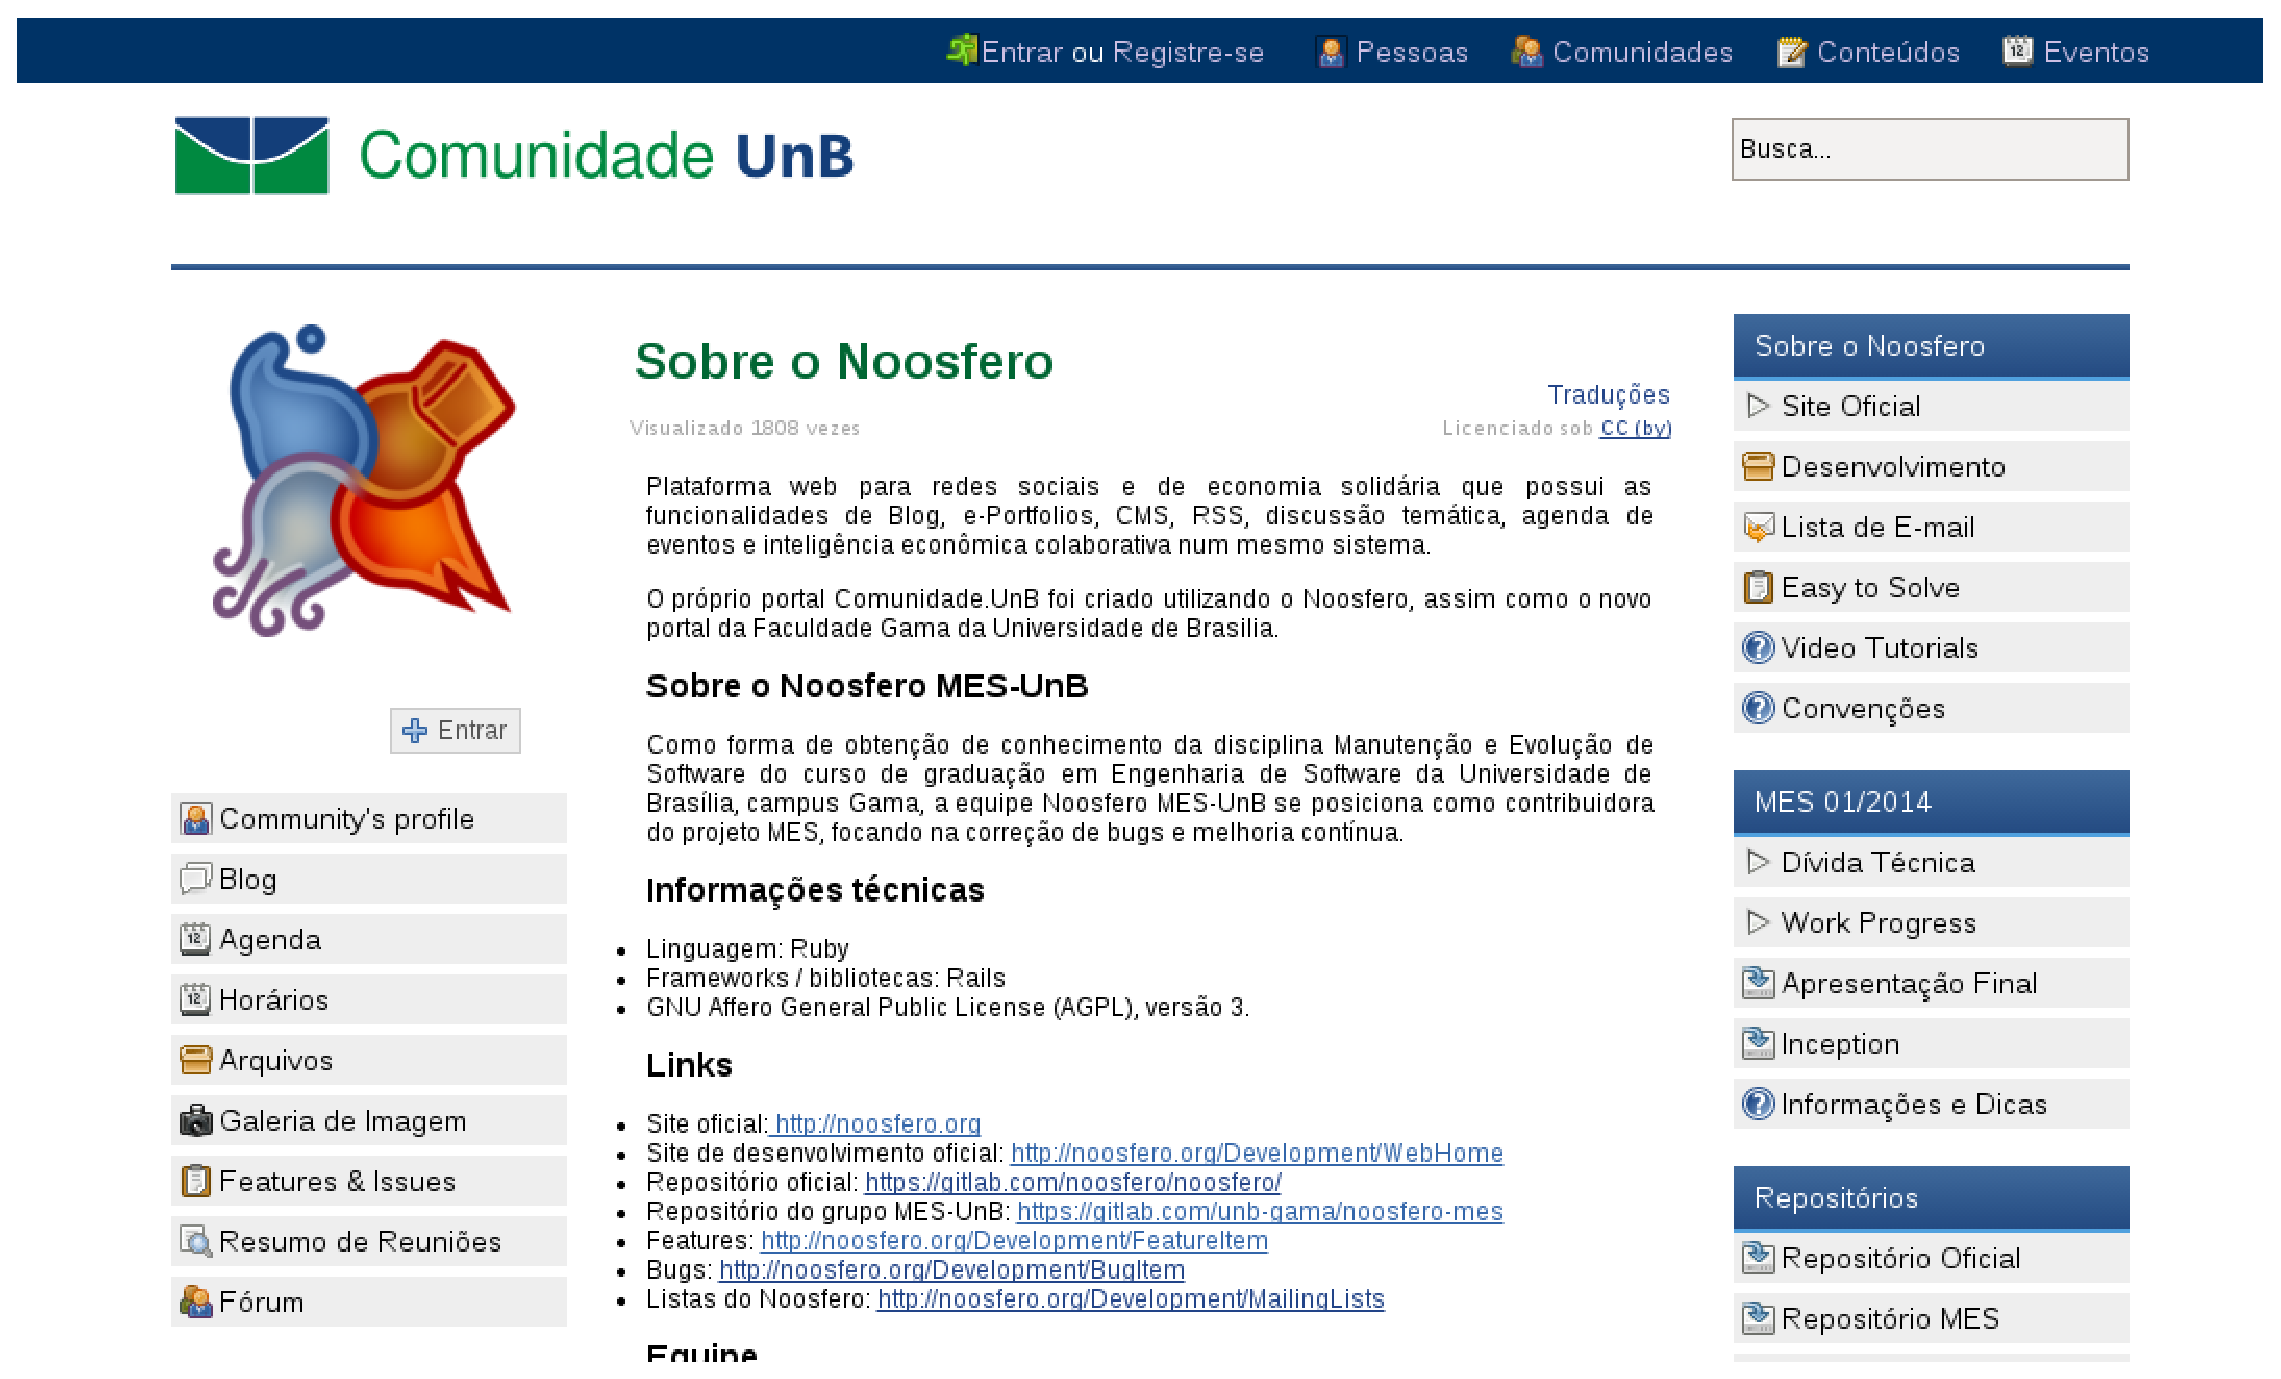
\includegraphics[keepaspectratio=true,scale=0.4]
      {figuras/comunidade-mes.eps}
    \caption{Exemplo do uso do Comunidade.UnB na disciplina de MES.}
    \label{comunidade-mes}
\end{figure}

Este é um exemplo de comunidade criada dentro do Comunidade.UnB, que possui características que se assemelham ao ambiente Moodle, como evidenciado na seção \ref{comparacao-ava}, carece de alguns funcionalidades importantes mas com a vantagem da possibilidade de acesso do público ao conteúdo, e a continuidade do conteúdo desenvolvido por outras pessoas que eventualmente se juntem ao longo do tempo. Vale lembrar que em uma publicação de conteúdo os níveis de privacidade podem ser alterados basicamente entre públicos e privados.

As limitações da plataforma e a proposta de uso da Comunidade.UnB por professores para a criação de disciplinas, estimulam o desenvolvimento de funcionalidades que levem à plataforma Noosfero a assemelhar-se a um ambiente virtual de aprendizagem. Desta maneira na seção \ref{desen-noosferAVA} é apresentada a proposta de estudo desse trabalho para desenvolvimento de funcionalidades e minimização das diferenças entre o Noosfero e os ambientes virtuais de aprendizegem.

\section{Desenvolvimento do NoosferAVA}
\label{desen-noosferAVA}

Nesta seção apresentaremos as funcionalidades que serão desenvolvidas para contribuir para a adequação do Noosfero a um ambiente virtual de aprendizagem, para exercer a função de apoio aos AVA adotados pela universidade. Serão apresentados os requisitos funcionais levantados para que esta possa suprir as necessidades levantadas.

Além das funcionalidades relatadas, julgou-se necessária a evolução do \textit{plugin Comunidade.UnB}, desenvolvido por \citeonline{bucher2013rede} com objetivo de integrar o Noosfero com o serviço de Lightweight Directory Access Protocol (LDAP). O LDAP é utilizado pela UnB para manter a base dados de todos os seus alunos e funcionários.

As funcionalidades serão apresentadas utilizando o formato de histórias de usuários uma vez que o Noosfero as utiliza no seu processo de desenvolvimento. Além disso os critérios de aceitação serão expostos no formato de cenários de uso, prática que é bastante conveniente ao Noosfero e é utilizada devido ao BDD.

% -Atualizar pro rails 3
\subsection{Evolução do \textit{plugin Comunidade.UnB}}
\label{plugin-comunidade}
% -realizar melhorias - cadastro de matricula dos usuários já existentes

O objetivo do \textit{plugin} do Comunidade.Unb é que o usuário tenha acesso através dos mesmos dados utilizados para acessar outros serviços, como, por exemplo, o serviço de matrícula \footnote{Disponível em: \url{https://matriculaweb.unb.br}} para alunos ou o serviço de lançamento de notas para professores.

A versão anterior do \textit{plugin} permitia que apenas os novos usuários realizassem o cadastro de suas matrículas, dessa maneira aqueles que já estavam cadastrados não tinham acesso ao portal. Devido as limitações de acesso definidas pelo \textit{plugin}, onde apenas usuários com matrícula cadastrada tem acesso ao sistema.

Foi criada nova versão do \textit{plugin} que permite cadastrar a matrícula dos usuários que já possuem registro no Comunidade.UnB. Dessa maneira o \textit{plugin Comunidade.UnB} poderá ser ativado permitindo a autenticação apenas dos usuários cadastrados no LDAP da universidade. Abaixo segue a história de usuário com seus respectivos cenários de uso.

\subsubsection*{Histórias de usuário}

% história
\begin{enumerate}
\item \underline{Autenticação via LDAP}

\textbf{Como} um aluno da Universidade Brasília

\textbf{Gostaria de} me autenticar na rede através da minha matrícula e senha

\textbf{Para} utilizar os mesmos dados de cadastro da UnB.

\subsubsection*{Cenários de uso:}

% cenário
\begin{enumerate}
\item \underline{Acesso sem matrícula cadastrada}

\textbf{[Dado]} que sou aluno da UnB

\textbf{[E]} possuo cadastro ativo na base de dados da UnB

\textbf{[E]} possuo cadastro ativo na base de dados do Comunidade.UnB

\textbf{[Quando]} eu acessar o portal

\textbf{Como} um aluno da Universidade Brasília

\textbf{[Então]} devo ser direcionado para uma página com o título ``Cadastrar Matrícula''

\textbf{[E]} devo ver os campos ``Matrícula'', ``Senha'' e
``confirmação de senha'' em branco.

\item \underline{Registro de matrícula de usuários existentes}

\textbf{[Dado]} que sou aluno da UnB

\textbf{[E]} me encontro na página de Cadastrar matrícula do Comunidade.UnB

\textbf{[Quando]} eu preencher os campos \\
``matrícula'' com ``100103979'',\\
e ``senha''  com a senha da base dados da UnB,\\
e ``confirmação de senha''

\textbf{[E]} clicar no botão ``Registrar''

\textbf{[Então]} eu devo ser direcionado para meu perfil
% cenários
\end{enumerate}
% histórias
\end{enumerate}

% -------------------- Evolução do Work Assignment ----------------
\subsection{Evolução do \textit{plugin Work Assignment}}

Nesta subseção serão apresentadas um primeiro levantamento das histórias correspondentes a evolução do \textit{plugin Work Assignment}. Até então o \textit{plugin} possui apenas a funcionalidade de permitir o envio de arquivos para o servidor em um determinado período de tempo.

A proposta de evolução é a criação de um sistema de notas que permita ao professor atribuir notas as atividades enviadas e dessa maneira acompanhar a situação de cada aluno. Do ponto de vista do aluno o mesmo poderá visualizar todas as notas das atividades em cada disciplina, avaliando se o seu desempenho está satisfatório.

Além disso é necessário uma evolução da funcionalidade que permite a definição do tempo restante para o envio, que atualmente é realizado de maneira manual não possibilitando o estabelecimento de intervalos de tempo.

\subsubsection*{Histórias de usuário}
% história
\begin{enumerate}
% ---------------------------------------------------------------------
\item \underline{Definir tempo restante}

\textbf{Como} um professor

\textbf{Gostaria de} definir o tempo restante para cada atividade no Work Assignment

\textbf{Para} gerenciar o envio de atividades pelos alunos em um determinado período.

\subsubsection*{Cenários de uso:}

\begin{enumerate}
\item \underline{Definir tempo}

\textbf{[Dado]} que esteja logado como professor

\textbf{[E]} selecione a o opção ``Gerenciar conteúdo''

\textbf{[Quando]} eu clicar em trabalho a ser entregue

\textbf{[Então]} devo visualizar a opção ``Ativar tempo de entrega''

\textbf{[E]} informar a data e hora máxima para envio da atividade.

\item \underline{Modificar tempo}

\textbf{[Dado]} que esteja logado como professor

\textbf{[E]} eu tenha atividades a ser entregue em aberto

\textbf{[E]} eu esteja visualizando as informações da atividade

\textbf{[Quando]} eu selecionar opção ``Editar''

\textbf{[E]} visualizar a opção ``Tempo de entrega''

\textbf{[Então]} deve ser permitido que eu altere o tempo definido

\textbf{[E]} visualize o resultado da alteração após a confirmação.

\item \underline{Permitir entrega de atividades após período}

\textbf{[Dado]} que esteja logado como professor

\textbf{[E]} selecione a o opção ``Gerenciar conteúdo''

\textbf{[E]} vavegar até a página trabalho a ser entregue

\textbf{[Quando]} selecionar a opção ``Ativar tempo de entrega''

\textbf{[Então]} devo visualizar a opção ``Permitir entrega após o período''

\textbf{[Para]} que eu possa selecioná-la.

\end{enumerate}
% -----------------------------------------------------------------------
\item \underline{Tempo restante de atividades}

\textbf{Como} um aluno

\textbf{Gostaria de} visualizar o tempo restante da atividade

\textbf{Para} enviar um arquivo na data correta.

\subsubsection*{Cenários de uso:}

\begin{enumerate}
\item \underline{Visualizar tempo}

\textbf{[Dado]} que esteja logado como Aluno

\textbf{[E]} eu esteja inscrito em um Curso

\textbf{[E possua atividade em aberto]}

\textbf{[Quando]} eu selecionar a opção de visualizar a atividade

\textbf{[Então]} eu devo visualizar se a atividade está em aberto

\textbf{[E]} qual o tempo restante para o envio da atividade.

\end{enumerate}

% -----------------------------------------------------------------------
\item \underline{Professor gerencia notas}

\textbf{Como} um professor

\textbf{Gostaria de} gerenciar as notas dos integrantes da comunidade

\textbf{Para} manter o controle sobre a pontuação de todos os alunos.

\subsubsection*{Cenários de uso:}

\begin{enumerate}

\item \underline{Definir grupo de atividades}

\textbf{[Dado]} que esteja logado como professor

\textbf{[E]} que a funcionalidade de notas eteja habilitada no plugin

\textbf{[E]} selecionar a opção ``Gerenciar notas''

\textbf{[E]} e eu selecionar o curso desejado

\textbf{[Quando]} eu clicar em ``Cadastrar grupo de atividades''

\textbf{[E]} eu preencho os campos \\
``Nome do grupo'',\\
e ``Lista de Atividades''\\
\textbf{[E]} eu clico em ``Salvar''

\textbf{[Então]} recebo uma mensagem de confirmação

\textbf{[E]} visualizo todas os grupos de atividades criados.

\item \underline{Visualizar notas de todos os alunos de uma determinada atividade}

\textbf{[Dado]} que esteja logado como professor

\textbf{[E]} que a funcionalidade de notas eteja habilitada no plugin

\textbf{[E]} selecionar a opção ``Gerenciar notas''

\textbf{[E]} e eu selecionar o curso desejado

\textbf{[Quando]} eu selecionar atividade

\textbf{[E]} algum aluno tenha enviado a atividade

\textbf{[Então]} devo visualizar todas as atvidades enviadas e suas respectivas notas.

\item \underline{Visualizar notas de todos ao alunos de um grupo de atividades}

\textbf{[Dado]} que esteja logado como professor

\textbf{[E]} que a funcionalidade de notas eteja habilitada no plugin

\textbf{[E]} selecionar a opção ``Gerenciar notas''

\textbf{[E]} e eu selecionar o curso desejado

\textbf{[Quando]} eu clicar em ``Visualizar notas por grupo de atividades''

\textbf{[E]} algum aluno tenha enviado a atividade

\textbf{[Então]} devo visualizar todas as atvidades daquele grupo e suas respectivas notas.

\end{enumerate}
% -----------------------------------------------------------------------

\item \underline{Atribuir notas aos alunos}

\textbf{Como} um professor

\textbf{Gostaria de} atribuir notas as atividades enviadas pelos alunos

\textbf{Para} avaliar o rendimento de cada um deles.

\subsubsection*{Cenários de uso:}

\begin{enumerate}
\item \underline{Atribuir notas}

\textbf{[Dado]} que esteja logado como professor

\textbf{[E]} que a funcionalidade de notas eteja habilitada no plugin

\textbf{[Quando]} selecionar uma atividade na lista de atividades

\textbf{[Então]} devo visualizar a opção atribuir nota

\textbf{[E]} devo visualizar o campo ``nota'' para preenche-lo.


\item \underline{Alterar notas}

\textbf{[Dado]} que esteja logado como professor

\textbf{[E]} que a funcionalidade de notas eteja habilitada no plugin

\textbf{[Quando]} selecionar uma atividade na lista de atividades

\textbf{[E]} atividade já possua notas

\textbf{[Então]} devo visualizar a opção alterar nota

\textbf{[E]} devo visualizar o campo ``nota'' para preenche-lo.

\end{enumerate}

% -----------------------------------------------------------------------

\item \underline{Publicar notas aos alunos}

\textbf{Como} um professor

\textbf{Gostaria de} publicar as notas atribuídas as atividades

\textbf{Para} que os alunos possam visualizar suas respectivas avalizações

\subsubsection*{Cenários de uso:}

\begin{enumerate}
\item \underline{Disponibilizar notas de uma determinada atividade}

\textbf{[Dado]} que esteja logado como professor

\textbf{[E]} que a funcionalidade de notas eteja habilitada no plugin

\textbf{[Quando]} selecionar uma atividade na lista de atividades

\textbf{[Então]} devo visualizar a opção ``permitir visualização''

\textbf{[E]} devo ter a opção de ativá-lo.

\item \underline{Omitir notas de uma determinada atividade}

\textbf{[Dado]} que esteja logado como professor

\textbf{[E]} que a funcionalidade de notas eteja habilitada no plugin

\textbf{[Quando]} selecionar uma atividade na lista de atividades

\textbf{[Então]} devo visualizar a opção ``permitir visualização''

\textbf{[E]} devo ter a opção de desativá-lo.

\end{enumerate}

% -----------------------------------------------------------------------
\item \underline{Aluno visualiza notas}

\textbf{Como} um aluno

\textbf{Gostaria de} visualizar minhas notas

\textbf{Para} inteira-me sobre minha pontuação nas atividades.

\subsubsection*{Cenários de uso:}
\begin{enumerate}

\item \underline{Visualizar cursos com notas disponíveis}

\textbf{[Dado]} que estou logado como ``Hebert''

\textbf{[E]} o plugin Work Assignment esteja ativo

\textbf{[E]} participo de alguma comunidade que utilize o plugin de notas

\textbf{[E]} existem notas de atividades disponíveis

\textbf{[E]} o professor tenha permitido sua visualização

\textbf{[Quando]} eu navegar até a página ``Minhas notas''

\textbf{[Então]} tenho que ver todos as comunidades (cursos) com notas disponíveis.

\item \underline{Detalhar notas de cada curso}

\textbf{[Dado]} que estou logado como ``Hebert''

\textbf{[E]} o plugin Work Assignment esteja ativo

\textbf{[E]} participo de alguma comunidade que utilize o plugin de notas

\textbf{[E]} existem notas de atividades disponíveis

\textbf{[E]} o professor tenha permitido sua visualização

\textbf{[E]} navegar até a página ``Minhas notas''

\textbf{[E]} visualizar todos as comunidades (cursos) com notas disponíveis

\textbf{[Quando]} eu selecionar a ``Visualizar detalhes'' de alguma comunidade

\textbf{[Então]} tenho que ver todos os grupos de atividades

\textbf{[E]} as notas disponibilizadas pelo professor.
% cenários
\end{enumerate}
% historia
\end{enumerate}

O desenvolviemnto desta funcionalidade é importante, pois segundo \citeonline[p. 37]{unb-professor} as notas para os alunos auxilia assimilação progressiva de conhecimento, e sabe-se que permite um maior \textit{feedback} para o aluno pois nem sempre fica transparente o seu desempenho ao longo do semestre. Colaborando ainda no quesito em que os AVA devem constituir de um gerenciamento pedagógico, que permita acesso e trabalho sobre os seguintes arquivos e estatísticas para controlar a evolução do estudante durante o curso \cite{pereira2007ambientes}.

As funcionalidades apresentadas neste capítulo irá colaborar para fazer uso do Comunidade.UnB se tornar um ambiente híbrido entre um ambiente virtual de aprendizagem e uma rede social para a troca de conhecimento através das comunidades e perfis de usuários. Permitindo englobar departamentos, organizações e projetos específicos da Universidade de Brasília.

\subsection{Pesquisa com alunos}
\label{pesquisa-alunos}

Afim de evidenciar a problematização e justificativa deste trabalho, realizou-se uma pesquisa junto aos alunos da FGA sobre o uso de redes sociais em seu dia a dia e sobre o seu uso para apoio as disciplinas cursadas na universidade. Para isso foi criado um questionário com quatro questões de múltipla escolha e para os itens associou-se a uma escala tipo \emph{Likert} de cinco pontos: Nunca; Raramente; Às vezes; (3) Frequentemente; Sempre (Instruções de preenchimento no Apêndice \ref{apen-inst}). Com esta escolha pode-se mapear todas as respostas seguindo a lógica em que há duas alternativas negativas, duas alternativas positivas e uma intermediária.

Nesta seção, apresentamos as questões elaboradas (Apêndice \ref{apen-quest}) e as respostas coletadas através da ferramenta \textit{Google Forms}. O questionário foi aplicado na rede social \textit{Facebook} em grupos específicos da FGA, foram coletadas e ao todo noventa e quatro respostas voluntárias ao questionário. Abaixo segue as questões com as respectivas análises de seus resultados, que estão representados graficamente no Apêndice \ref{apen-quest-result}.

\subsection*{Com que frequência você utiliza redes sociais?}

A primeira pergunta tinha como objetivo levantar com que frequência os alunos utilizam as redes sociais. Na Figura \ref{pergunta1} nota-se que 98\% dos alunos que responderam ao questionário utilizam as redes sociais sempre ou frequentemente, o que evidencia o fato que atualmente os estudantes dessa geração estão inseridos neste contexto.

\subsection*{Você utiliza alguma rede social como ferramenta de apoio as disciplinas?}

O intuito da segunda pergunta foi verificar se os alunos utilizam alguma ferramenta de redes social como ferramenta de apoio as disciplinas. Na Figura \ref{pergunta2} verifica-se que apenas 16\% dos alunos às vezes utilizam e de outro ponto de vista 83\% dos alunos fazem uso da rede para tal. Demonstrando que mesmo a universidade utilizando AVA os alunos se apoiam em redes sociais para discutir e compartilhar conteúdos referentes as disciplinas cursadas.

\subsection*{Os professores incentivam o uso de redes sociais para suas disciplinas?}
% 11\% Sempre
% 19\% frequentemente
% 52\% Ás vezes
% 17\% Raramente
% 1\% Nunca

O objetivo desta pergunta foi verificar se mesmo que a universidade indique o uso de AVA se os professoes incentivam o uso das redes sociais em suas disciplinas. Na Figura \ref{pergunta3} percebe-se que pouco mais da metade dos alunos (52 \%) tem suas respostas em um ponto intermediário do questionário, mostrando que os professoes são bem imparciais quanto a isso. Apesar que do restante, tem-se mais respostas favoráveis do que contra.

\subsection*{Mesmo que o professor não recomende o uso de redes sociais para discussão de conteúdos de suas disciplinas, você as utiliza?}
% 30\% Sempre
% 45\% frequentemente
% 20\% Ás vezes
% 4\% Raramente
% 0\% Nunca

Na quarta e última pergunta buscou-se investigar se os alunos utilizam as redes sociais como uma ferramenta de apoio as disciplinhas mesmo que os professores não recomende seu uso para tal. Dos que responderam 75\% não levam em consideração tais recomendações e fazem o uso, demonstrando que os alunos preferem estar nas redes sociais onde expõem suas opiniões a fim de promover o compartilhamento de conteúdo (Resultados na Figura \ref{pergunta4}).
